\documentclass[border=10pt]{standalone}
\usepackage{lmodern}
\usepackage[T1]{fontenc}
\usepackage{amsmath}
\usepackage{booktabs}
\usepackage{tikz}
\usepackage{xcolor}

\definecolor{drivcol}{HTML}{7AB648}
\definecolor{posternavy}{HTML}{1B2A4A}

\begin{document}

\begin{tikzpicture}
\node[draw=drivcol!80!black, fill=drivcol!10, rounded corners=6pt, line width=0.8pt,
      inner sep=0.8em, text width=28cm] {%

\textsf{\textbf{\Large CRPS \& CRPSS --- reference (not on poster)}}

\vspace{0.6em}

{\small All formulas are for \textbf{one gridpoint, one lead week, one initialisation}. Each value ($f_j$, $o$, $c$) is a weekly mean temperature in \textdegree C. Subscript $j$ indexes ensemble members ($j = 1,\ldots,M$): there are 11 forecast values but only \textbf{one} observed value, so $o$ has no member subscript.}

\vspace{1em}

%--- Step 1: Regular CRPS ---
\textsf{\textbf{Step 1: Regular CRPS (unfair)}}
\vspace{0.4em}

\begin{tikzpicture}
\node[draw=posternavy!50, fill=white, rounded corners=4pt, line width=0.6pt,
      inner sep=0.6em, text width=26.5cm] {%
\begin{minipage}[c]{0.60\linewidth}
$\displaystyle
\text{CRPS} \;=\; \underbrace{\frac{1}{M}\sum_{j=1}^{M}\left|f_j - o\right|}_{\text{MAE term}} \;-\; \underbrace{\frac{1}{2M^{\mathbf{2}}}\sum_{j=1}^{M}\sum_{k=1}^{M}\left|f_j - f_k\right|}_{\text{spread term}}
$
\end{minipage}%
\hfill
\begin{minipage}[c]{0.37\linewidth}
{\footnotesize
\begin{tabular}{@{}r@{\;=\;}l@{}}
$f_j$ & weekly mean of ensemble member $j$ \\
$o$ & weekly mean of ERA5 observation \\
$M$ & ensemble size (11 for EEFH) \\
\end{tabular}

\vspace{0.3em}

The spread term is the mean pairwise distance between all members. Intuition: how wide is the ensemble?
}
\end{minipage}%
};
\end{tikzpicture}

\vspace{0.3em}
{\small \textbf{Problem:} with finite $M$, the double sum underestimates the true spread (you're sampling 11 members from a continuous distribution, so you miss the tails). Smaller ensembles get penalised more.}

\vspace{1em}

%--- Step 2: Fair CRPS ---
\textsf{\textbf{Step 2: Fair CRPS (Ferro 2014) --- what we actually compute}}
\vspace{0.4em}

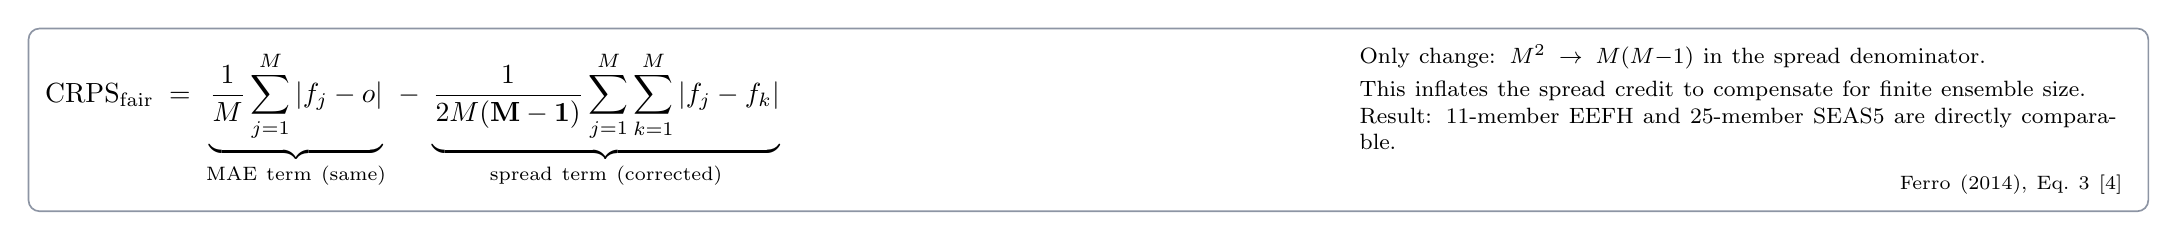
\begin{tikzpicture}
\node[draw=posternavy!50, fill=white, rounded corners=4pt, line width=0.6pt,
      inner sep=0.6em, text width=26.5cm] {%
\begin{minipage}[c]{0.60\linewidth}
$\displaystyle
\text{CRPS}_{\text{fair}} \;=\; \underbrace{\frac{1}{M}\sum_{j=1}^{M}\left|f_j - o\right|}_{\text{MAE term (same)}} \;-\; \underbrace{\frac{1}{2M\mathbf{(M-1)}}\sum_{j=1}^{M}\sum_{k=1}^{M}\left|f_j - f_k\right|}_{\text{spread term (corrected)}}
$
\end{minipage}%
\hfill
\begin{minipage}[c]{0.37\linewidth}
{\footnotesize
Only change: $M^2 \;\to\; M(M{-}1)$ in the spread denominator.

\vspace{0.3em}

This inflates the spread credit to compensate for finite ensemble size. Result: 11-member EEFH and 25-member SEAS5 are directly comparable.

\vspace{0.3em}
\hfill{\scriptsize Ferro (2014), Eq.~3 [4]}
}
\end{minipage}%
};
\end{tikzpicture}

\vspace{0.3em}
{\small \textbf{Equivalent sorted form} (what the code uses, faster to compute):
$\;\displaystyle\text{CRPS}_{\text{fair}} = \frac{1}{M}\sum_{j=1}^{M}|f_j - o| \;-\; \frac{1}{M(M-1)}\sum_{j=1}^{M}(2j - M - 1)\,f_{(j)}$
\;\;where $f_{(j)}$ = members sorted ascending.}

\vspace{1.2em}

%--- Step 3: CRPSS ---
\textsf{\textbf{Step 3: CRPSS --- skill relative to climatology}}
\vspace{0.4em}

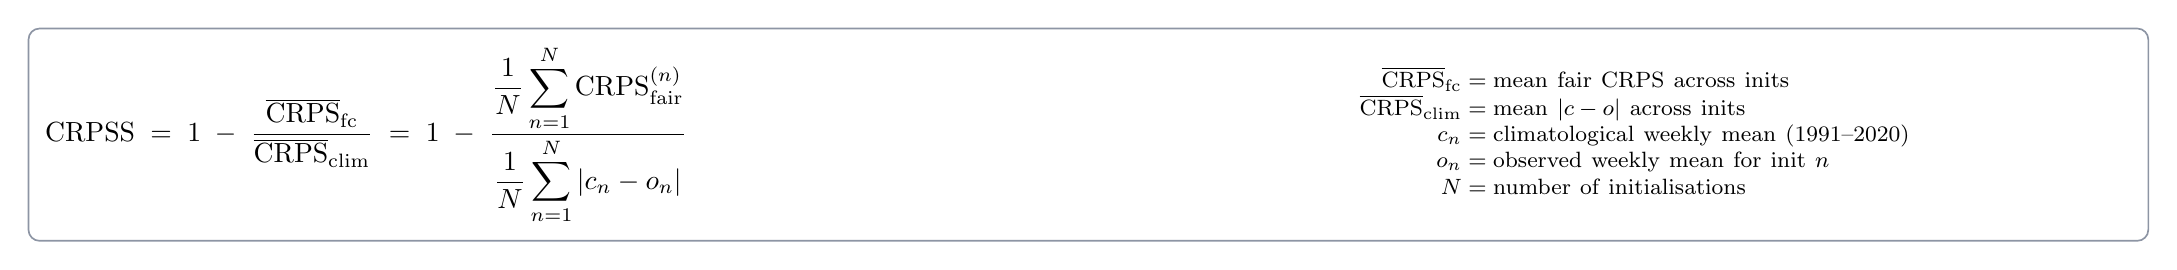
\begin{tikzpicture}
\node[draw=posternavy!50, fill=white, rounded corners=4pt, line width=0.6pt,
      inner sep=0.6em, text width=26.5cm] {%
\begin{minipage}[c]{0.60\linewidth}
$\displaystyle
\text{CRPSS} \;=\; 1 \;-\; \frac{\overline{\text{CRPS}}_{\text{fc}}}{\overline{\text{CRPS}}_{\text{clim}}}
\;=\; 1 \;-\; \frac{\displaystyle\frac{1}{N}\sum_{n=1}^{N}\text{CRPS}_{\text{fair}}^{(n)}}{\displaystyle\frac{1}{N}\sum_{n=1}^{N}\left|c_n - o_n\right|}
$
\end{minipage}%
\hfill
\begin{minipage}[c]{0.37\linewidth}
{\footnotesize
\begin{tabular}{@{}r@{\;=\;}l@{}}
$\overline{\text{CRPS}}_{\text{fc}}$ & mean fair CRPS across inits \\
$\overline{\text{CRPS}}_{\text{clim}}$ & mean $|c - o|$ across inits \\
$c_n$ & climatological weekly mean (1991--2020) \\
$o_n$ & observed weekly mean for init $n$ \\
$N$ & number of initialisations \\
\end{tabular}
}
\end{minipage}%
};
\end{tikzpicture}

\vspace{0.3em}
{\small \textbf{Why $|c_n - o_n|$ for climatology?} Climatology is a single value ($M{=}1$). With one ``member'', the spread term has $M(M{-}1) = 0$ in the denominator and vanishes. CRPS for a deterministic forecast $=$ absolute error. So the reference is just: how far is the long-term average from the truth?}

\vspace{1.2em}

%--- Interpretation ---
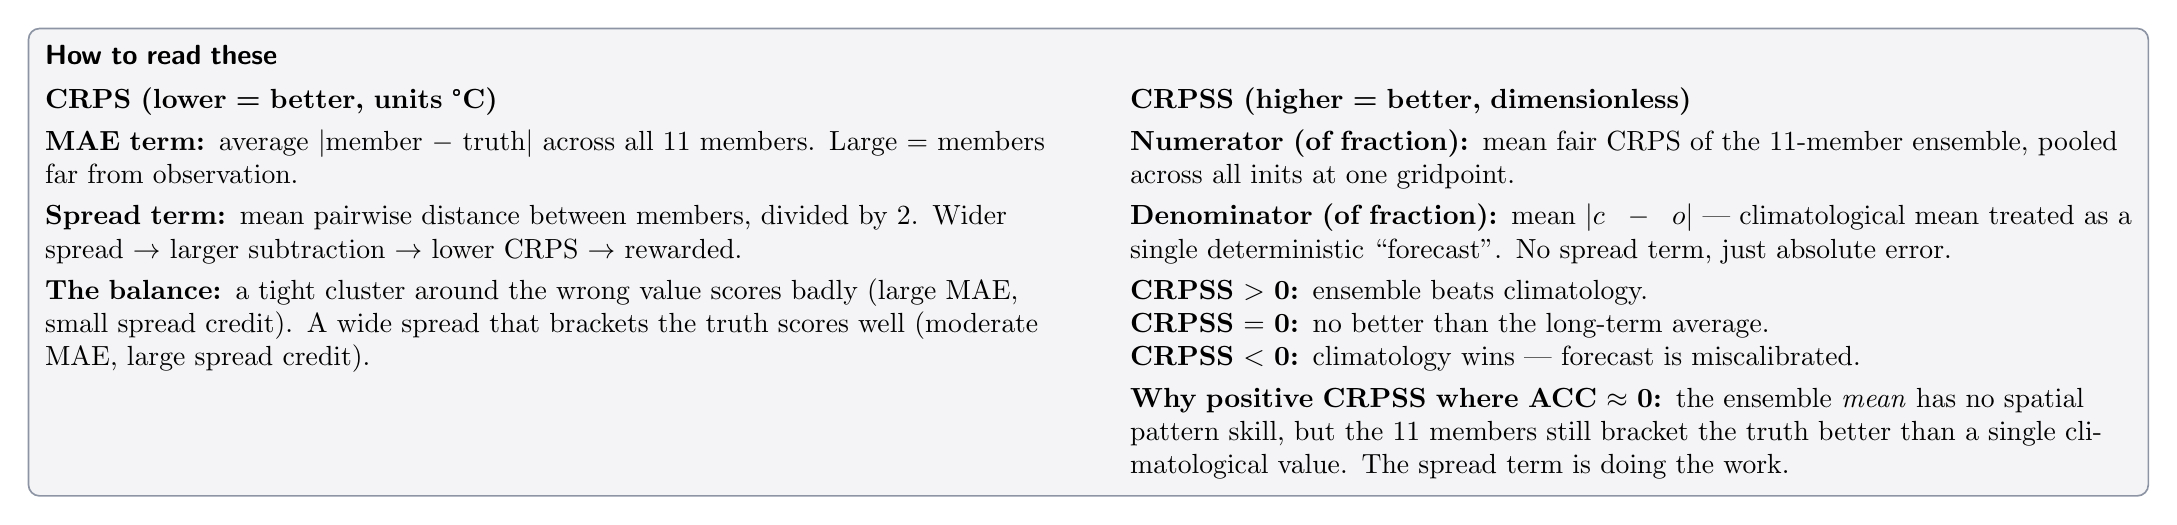
\begin{tikzpicture}
\node[draw=posternavy!50, fill=posternavy!5, rounded corners=4pt, line width=0.6pt,
      inner sep=0.6em, text width=26.5cm] {%
\textsf{\textbf{How to read these}}

\vspace{0.4em}

\begin{minipage}[t]{0.48\linewidth}
\textbf{CRPS (lower = better, units \textdegree C)}

\vspace{0.3em}

\textbf{MAE term:} average $|$member $-$ truth$|$ across all 11 members. Large $=$ members far from observation.

\vspace{0.3em}

\textbf{Spread term:} mean pairwise distance between members, divided by 2. Wider spread $\rightarrow$ larger subtraction $\rightarrow$ lower CRPS $\rightarrow$ rewarded.

\vspace{0.3em}

\textbf{The balance:} a tight cluster around the wrong value scores badly (large MAE, small spread credit). A wide spread that brackets the truth scores well (moderate MAE, large spread credit).
\end{minipage}%
\hfill
\begin{minipage}[t]{0.48\linewidth}
\textbf{CRPSS (higher = better, dimensionless)}

\vspace{0.3em}

\textbf{Numerator (of fraction):} mean fair CRPS of the 11-member ensemble, pooled across all inits at one gridpoint.

\vspace{0.3em}

\textbf{Denominator (of fraction):} mean $|c - o|$ --- climatological mean treated as a single deterministic ``forecast''. No spread term, just absolute error.

\vspace{0.3em}

\textbf{CRPSS $>$ 0:} ensemble beats climatology.\\
\textbf{CRPSS $=$ 0:} no better than the long-term average.\\
\textbf{CRPSS $<$ 0:} climatology wins --- forecast is miscalibrated.

\vspace{0.3em}

\textbf{Why positive CRPSS where ACC $\approx$ 0:} the ensemble \textit{mean} has no spatial pattern skill, but the 11 members still bracket the truth better than a single climatological value. The spread term is doing the work.
\end{minipage}%
};
\end{tikzpicture}

};
\end{tikzpicture}

\end{document}
